\section{Mobile cellular networks until the forth generation}\label{sec:redesMoveis}

While the word `cellular' has become almost redundant nowadays when referring to mobile networks, it summarizes several concepts and innovations. A mobile radio (telephone) service was initially provided by high-power transmitters/receivers that could communicate directly to each other until a radius of about 80~km. These devices were heavy, expensive, consumed a lot of energy, and, as expected, had no support for data communication. The introduction of the cellular radio changed the scenario drastically, allowing the development of small, cheap, energy-efficient, and, later, data-oriented communication devices. Since the first commercial mobile cellular network, in 1979, until nowadays, several new technologies have been introduced in the communication systems, but also several concepts remain the same or are very similar. In this section, we present relevant concepts of mobile networks in general and the ones related to cellular networks. Additionally, we describe the history of the mobile cellular networks very briefly through the `generations', starting from the first until the fourth, with most of the attention to the fourth generation. The fifth-generation and beyond have the next section dedicated to them.


\subsection{Basic concepts}

The fundamental idea of a cellular network is the use of multiple low-power transceivers (transmitters+receivers) to offer communication to mobile devices. Actually, the power of these transceivers is low compared with their predecessors, but it is very high compared with mobile devices. Traditionally, these transceivers are mounted in a mast or tower, at an elevated point, and have a control unit. This configuration is named as a Base Station or BS, which is responsible for covering an area using a band of frequencies. Assuming the most traditional positioning in the center of the coverage area, the area's conceptual representation as a hexagon was the appropriate choice because the distance between the centers of all adjacent areas is the same (equal to $\sqrt{3}R$). Therefore, a mobile cellular network can be represented as a collection of the neighboring regions, each resembling a cell, as illustrated in Fig.~\ref{subfig:cell_net_ideal}. In practice, the environmental characteristics and the propagation conditions tend to degenerate the mobile cellular network into something more similar to a Voronoi diagram or tessellation, as illustrated in Fig.~\ref{subfig:cell_net_practice}.

\begin{figure}[htb]
\centering
    \subfigure[Ideal]
    {\label{subfig:cell_net_ideal}
    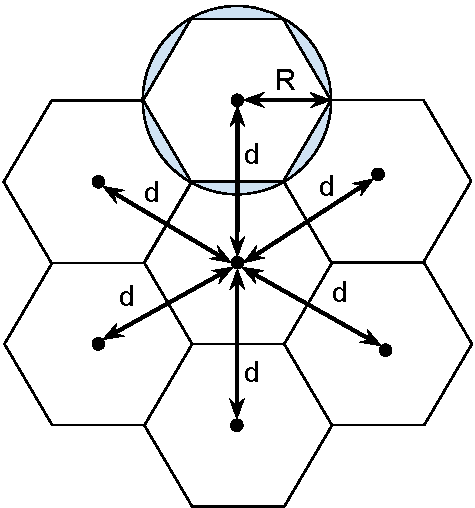
\includegraphics[width=.32\textwidth]{figs/cell_net_ideal.pdf}}
    \hfil
    \subfigure[Practical (positions randomly generated in GNU Octave)]
    {\label{subfig:cell_net_practice}
    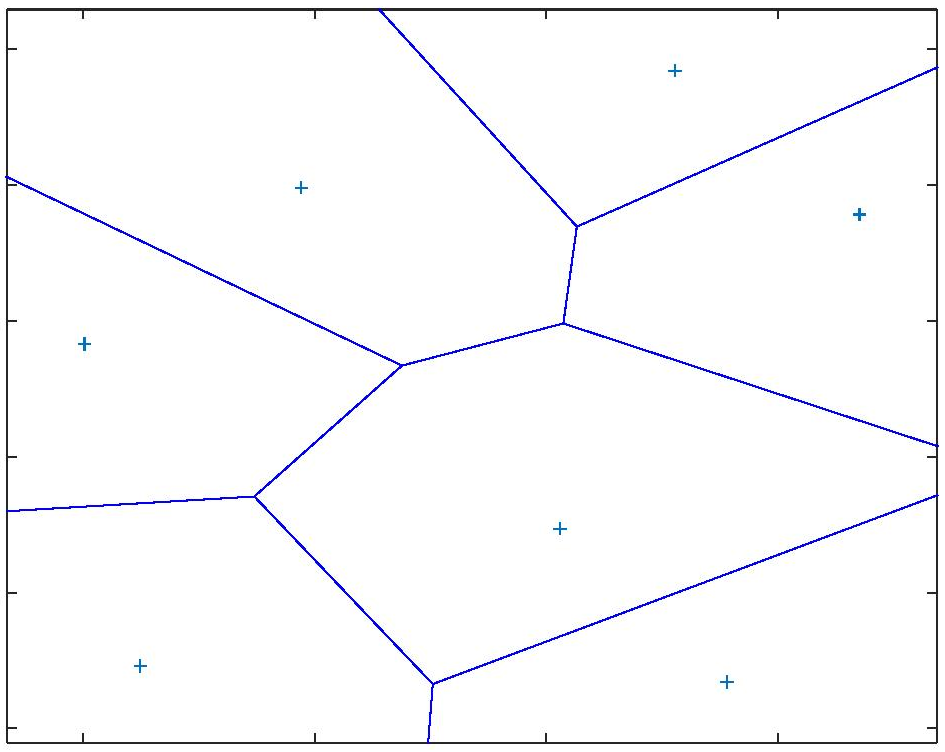
\includegraphics[width=.32\textwidth]{figs/cell_net_practice.pdf}}
    \caption{Representation of a cellular network.}
\label{fig:cell_net}
\end{figure}

The deployment of the BSs is generally defined by a previous study that takes into consideration factors as topographical characteristics, signal propagation conditions, limitations on siting antennas, and demand of the users. While in-site measurements are common, most of the study is generally performed with propagation models that can estimate the signal power received along the whole covered are. These models try to represent in a very compact way the complex propagation dynamics of the wireless signal. Table~\ref{tab:prop_models} lists a small set of models available in the literature and their frequency ranges.

\begin{table}[htb]
\centering
%\footnotesize
\begin{tabular}{ll}
\hline
\textbf{Model} & \textbf{Frequency range}  \\
\hline
Okumura-Hata & 150--1500~MHz\\
COST 231 -- Walfish-Ikegami & 800--2000~MHz\\ 
ITU-R P.529 & 700--3500~MHz \\ \hline
\end{tabular} 
\caption{Examples of propagation models.}
\label{tab:prop_models}
\end{table}

Traditionally, a mobile cellular network operates in licensed bands which must be acquired according to the specific set of rules of each country and may be very expensive. Therefore, a lot of the effort is devoted to managing the frequencies available for communication properly. This management involves several coordinated approaches to seek the efficient usage of the Radio Frequency (RF) spectrum, which include antenna schemes, power control, interference control, frequency reuse, among others.

While all these concepts are still relevant in modern cellular networks, new concepts and technologies such as Multiple-Input Multiple-Output (MIMO), beamforming, and millimeter-wave communications have a significant impact. For example, beamforming makes it more complex to define cell coverage and also to identify interference. Communications in the millimeter-wave bands (\textit{i.e.}, above 24~GHz) have very different propagation characteristics than the traditional sub-6~GHz employed along decades in the mobile-cellular networks.

\subsection{Basic operation of a cellular system}

In its original configuration, a cellular system could be summarized into the following elements: Mobile Telecommunications Switching Office (MTSO), BS, and mobile unit or User Equipment (UE). Fig.~\ref{fig:cell_system} illustrates a basic cellular system. In a modern cellular system, the MTSO can be identified as the core (network), while the collection of BSs is named as Radio Access Network (RAN). Actually, several other elements are composing the core and RAN, as we describe later in this and the following sections.

\begin{figure}[htb]
 \begin{center}
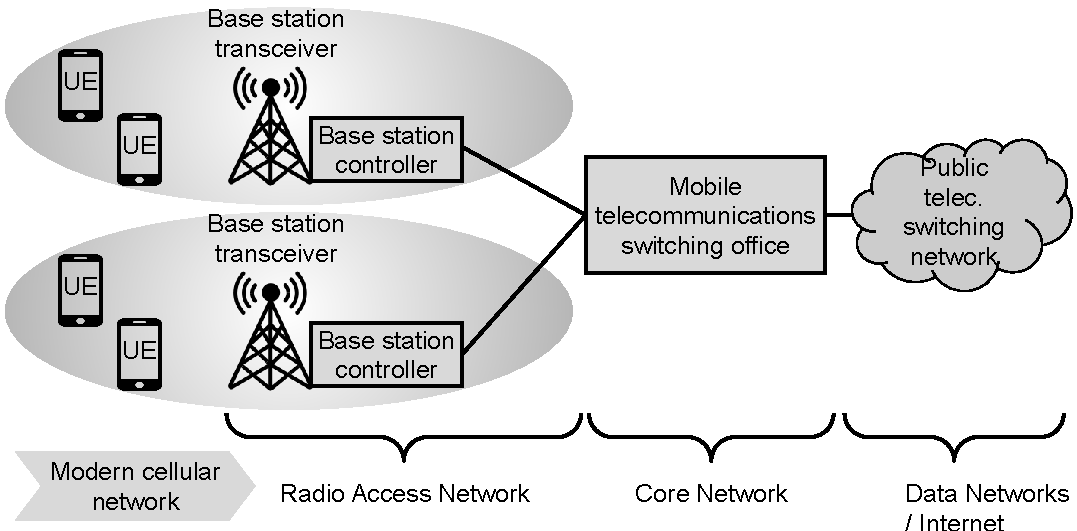
\includegraphics[width=0.5\textwidth]{figs/cell_system.pdf}
  \end{center}
\caption{Overview of a basic cellular system.}
\label{fig:cell_system}
\end{figure}

The BS controller handles the communication process between the UE and the rest of the network. Each BS may simultaneously serve multiple UEs under its coverage area. One MTSO serves multiple BSs, being connected generally through wired links, but wireless links are also common. Traditionally, all communications between UEs are established through a BS, even when they are close to each other. The concepts, technologies, and standards for direct communication (known as device-to-device or D2D~\cite{kar:18}) between UEs have already been introduced in cellular networks. However, when its effective adoption begins, it remains uncertain. An MTSO connects to the public telephone or telecommunications network, offering interconnection between its UEs and the outside networks. Several other management tasks are performed by an MTSO to assist its UEs, such as channel (de)allocation, handoff, paging, monitoring, and billing.

The channel (de)allocation may occur in different situations, for example, when UE is turned on or off, when UE moves from one BS coverage to another, if UE has a signal too weak, among others. The handoff process consists of the coordinated transfer of UE communication while moving between neighboring BSs, involving signal monitoring and channel allocation and deallocation. The paging process consists of finding a UE that has not been communicating for some time and so its location is unknown. Generally, the paging process is started by an incoming communication to UE. In addition to the wireless signal quality, the cellular network also monitors the traffic of UEs to charge the users properly. All these procedures remain in modern mobile networks, naturally, more focused on data instead of voice. Furthermore, technological advances imply updating some concepts. For example, instead of channel allocation and deallocation, modern mobile networks may allocate and deallocate Physical Resource Blocks (PRBs) and millimeter-wave beams, and even edge computing resources.

Similar to the traditional telecommunication systems, in a cellular system, the only concerns of a user are to initiate or answer a communication. The network system transparently manages everything, \textit{i.e.}, the user does not need to worry about configuration, reconfiguration, tuning, or any related task. Similar to traditional telecommunication systems, a cellular system has two types of channels between UEs and BSs: control and traffic channels. Control channels are used to exchange information related to control and management tasks (\textit{e.g.}, UE initialization, handoff, paging). Traffic channels are used to transport (voice or data) communications. In modern cellular networks, a more generic nomenclature is adopted, control plane, and user plane, but the meaning is very similar.

\subsection{Evolution of the mobile cellular networks}

By employing the arguable separation in `generations', the characteristics of the mobile cellular networks, until the fourth generation, can be loosely summarized by the information presented in Table~\ref{tab:geracoes}. A detailed description of the history of mobile cellular networks can be found in~\cite{stallings2014data,schiller2003mobile}, since our concerns are only the main characteristics of each generation and their relationship with the softwarization process. Naturally, the fourth generation deserves special attention since it is the first one designed to have data and software as relevant elements and also due to its present market share.

\begin{table*}[tbh]
\centering
\begin{threeparttable}
\begin{tabular}{lcccc}
\hline
\textbf{}      & \textbf{1G}   & \textbf{2G} & \textbf{3G}                         & \textbf{4G}    \\ \hline
Deployment  & $\approx1980$          & $\approx1991$        & $\approx1999$     & $\approx2009$  \\ 
Main services       & Analog voice & Digital voice, SMS & Digital voice, data packets & IP packets \\ 
Data rate  & 1.9 kbps      & 14.4 kbps   & 384 kbps                            & 200 Mbps       \\ 
%Multiplexação  & FDMA          & TDMA, CDMA  & TDMA, CDMA                          & OFDMA, SC-FDMA \\ 
RAN &   \begin{tabular}[c]{@{}c@{}}AMPS, TACS, NMT,\\ C-450, TMA, RTM\end{tabular}   &   \begin{tabular}[c]{@{}c@{}}GSM, GPRS, EDGE,\\PDC, IS-95, IS-136\end{tabular} & \begin{tabular}[c]{@{}c@{}}UMTS (W-CDMA),\\ CDMA2000, TD-SCDMA \end{tabular}  &  LTE, WiMAX
\\ 
Core & PSTN (SS7)        & PSTN (SS7, ISDN)   & PSTN, ATM, IP     & IP network (EPC)            \\ 
3GPP initial standard           &      -         &       -      &      Release 99 &  Release 8         \\
Global market share (by 2019)\tnote{1} & 0\% & 23\% & 25\% & 52\% \\ \hline
\end{tabular}
\begin{tablenotes}
\item[1] \url{https://www.statista.com/statistics/740442/worldwide-share-of-mobile-telecommunication-technology/}
\end{tablenotes}
\caption{Characteristics of the generations of the cellular networks.}
\label{tab:geracoes}
\end{threeparttable}
\end{table*}

Nowadays, 1G is the only one without commercial deployments in operation, while the other generations still exhibit a significant presence. For example, 2G, with the lowest participation, still has more than 20\% of the market share. The substantial investment in the legacy hardware and new opportunities, such as the support for IoT communications, can partially explain the long-living of 2G and 3G networks. Until the 3G, there was a considerable fragmentation in the radio access technologies, which is illustrated by the several standards available. A large number of players and the trade-offs of the competing technologies are some characteristics of the maturity level of the cellular networks at that time and helps to explain the fragmentation scenario. By the end of 2G and the beginning of 3G, the 3GPP initiative was introduced, having great success in 3G and 4G. The fourth-generation is the first focused on data communication. It offers, by design, proper support for the IP (Internet Protocol) stack and notably higher data rate in comparison with the previous generation.

\subsubsection*{First generation -- 1G}

The first commercially deployed cellular networks, now labeled as 1G, were an extension of the Public Switched Telephone Network (PSTN). Therefore, the focus was on analog voice communication, without any concern about data communication. Later, the network infrastructure was adapted to transport data but achieving only very low rates. The software in this generation was proprietary, low-level, and embedded in specific hardware. The network control was digital, but voice communication was analog. Despite the several limitations, the first-generation cellular networks were a great success, motivating the evolution and giving rise to a high-valuable and strategic industry.

\subsubsection*{Second generation -- 2G}

Compared with 1G, the second-generation cellular networks provided higher-quality signals, higher data rates, and greater capacity. 2G introduced digital traffic channels, \textit{i.e.}, 2G systems support digital data natively, and voice is digitally encoded before transmitting. Since all information becomes digital, 2G systems started offering support for encrypting both user and control traffic. The digital traffic also allows the adoption of error detection and correction techniques, which improves the quality of voice communication. 2G systems also introduced new services, such as the Short Message Service (SMS), that was very successful. Time-Division Multiple Access (TDMA) and Code Division Multiple Access (CDMA) were also introduced, improving efficiency in the use of the RF spectrum. While bit rates offered by 2G networks are too slow for many modern applications, they are suited for a wide range of IoT demands. This suited possibility has motivated infrastructure operators around the world to extend the life of 2G systems and vendors to revisit some products to improve relevant performance metrics for IoT, such as energy efficiency.

The software in 2G systems already had an important role, being responsible for the critical control and management tasks, including monitoring and billing. However, proprietary technologies and specialized appliances, \textit{i.e.}, combined hardware and software, were dominant. On the other hand, the adoption of solutions based on standards for open systems, such as the Telecommunications Management Network (TMN) defined by ITU-T, may be seen as initial steps to a more advanced softwarization process in the telecommunication area. In 2G systems, Global System for Mobile Communications (GSM) had great success, and, nowadays, some open-source software projects implement enough GSM features to have a basic operational cellular network. For example, OpenBTS and YateBTS\footnote{OpenBTS: \url{http://openbts.org/}; YateBTS: \url{https://yatebts.com/}} offer open-source software for the Base Transceiver Station (BTS), while OsmocomBB\footnote{https://osmocom.org/projects/baseband} implemented an open-source GSM baseband software.

\subsubsection*{Third generation -- 3G}

The benefits introduced by the second generation expanded the global deployment and the interest of the general public in mobile networks. In the early 90s, the ITU requested proposals for radio transmission technologies as part of the International Mobile Telecommunications (IMT) 2000 program. This program planned to have a universal global system, but after many discussions and disputes about patents, a family of 3G standards was adopted. 3GPP, for the Universal Mobile Telecommunications System (UMTS), and 3GPP2\footnote{3GPP2 is not an evolution of 3GPP, but a different standardization body.}, for the CDMA2000, became the main driving forces in the third generation's standardization process. Release 99 is the initial set of 3G UMTS standards published by 3GPP and the last one numbered according to the standardization year (or close since it was finished in 2000). The next is Release 4 that describes the UMTS all-IP Core Network.

In comparison with 2G, the third-generation cellular networks increased the data rates, improved the quality of voice communication, improved the efficiency in the use of the RF spectrum, enhanced the integration with IP networks, and enhanced the support for new services. However, 3G still maintains backward compatibility with several previous technologies, \textit{e.g.}, circuit switch is always supported. Although incompatible variants multiple have been adopted, CDMA was largely evolved in 3G and became the dominant technology for wireless communication in that generation. The software in 3G systems become even more relevant than in the previous generation since the infrastructure is more complex, and data communication becomes more relevant. However, proprietary software and vendor-specific appliances protected by endless patents increase the costs and delay innovation. On the other hand, in the first years of the millennium, mobile cellular networks were already essential, so the evolution of these systems became unstoppable.

Similar to 2G, 3G also may have its life extended due to IoT and also due to the more recent and significant investments. During the deployment of 3G, the telecommunication sector faced an economic world crisis and expensive auctions for obtaining the RF spectrum. UMTS was the most successful standard in 3G and, similar to GSM, has some open-source software, provided by the same developer groups. OpenBTS-UMTS\footnote{\url{https://github.com/RangeNetworks/OpenBTS-UMTS}} implements the basic functionalities according to the Release 99, using OpenBTS as a framework. The project Cellular Network Infrastructure\footnote{\url{https://projects.osmocom.org/projects/cellular-infrastructure/}} from Osmocom offers a complete implementation that allows for deploying an operational 3G system.

\subsubsection*{Fourth generation -- 4G}

The first billion of mobile subscribers was passed in 2002, the second billion in 2005, the third billion in 2007, the fourth billion by the end of 2008, and the fifth billion in 2010~\cite{holma2011lte}. During that decade, the volume of data traffic increased notably, until the global mobile data traffic surpassed voice by the end of 2009\footnote{\url{https://www.ericsson.com/en/press-releases/2010/3/mobile-data-traffic-surpasses-voice}}. Therefore, the plans for evolving the mobile cellular networks into the fourth generation needed to be aggressive to catch up with the demand and data-oriented characteristic. In 2002, the work on IMT-Advanced started by seeking to define the vision and requirements for the next generation of mobile cellular networks. The ``VAN diagram'', introduced by the ITU~\cite{itu:03} and replicated in Fig.~\ref{fig:imt-adv}, summarizes some initial ideas for the fourth generation. In addition to the very high data rates for both mobile and fixed/nomadic users, the IMT-Advanced also identified several other requirements, including the following:
\begin{itemize}
    \item Employ an all-IP packet switched network.
    \item Dynamically share the network resources to support more simultaneous users per cell.
    \item Support smooth handovers across heterogeneous networks.
    \item Offer high quality of service for multimedia applications.
\end{itemize}

\begin{figure}[htb]
 \begin{center}
    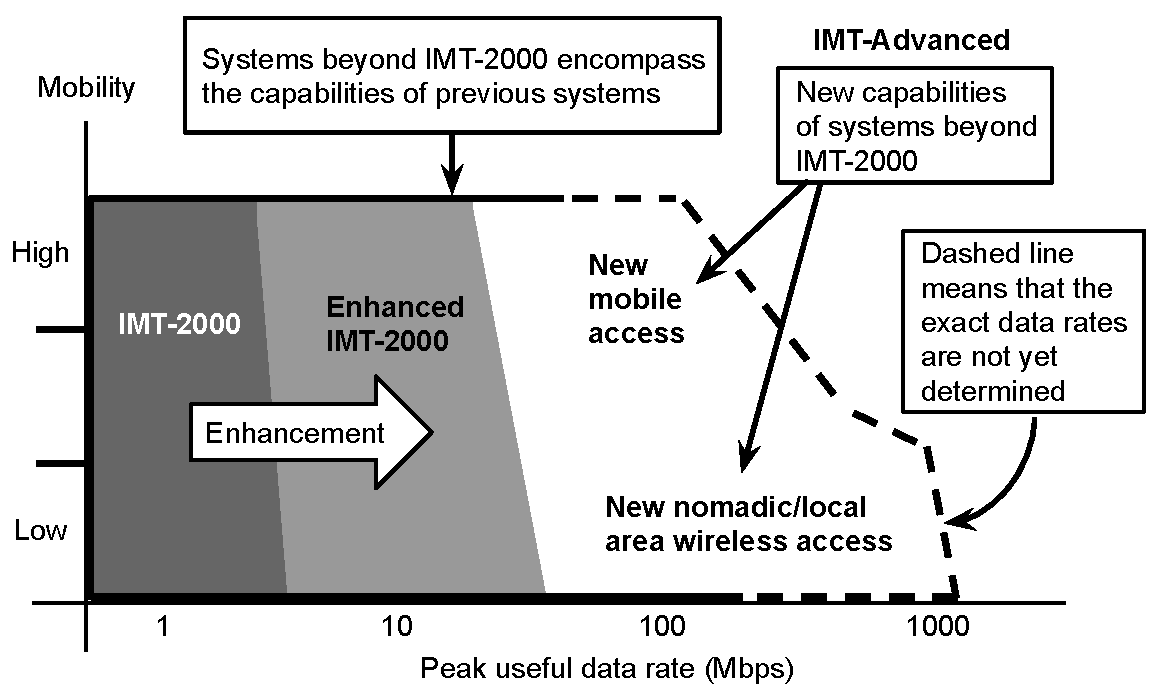
\includegraphics[width=0.5\textwidth]{figs/imt-adv.pdf}
  \end{center}
\caption{IMT-2000 capabilities and systems beyond IMT-2000.}
\label{fig:imt-adv}
\end{figure}

In 2009, only two candidate proposals for IMT-Advanced were submitted to ITU: 3GPP LTE-Advanced (LTE-A) and IEEE 802.16m (Mobile WiMAX Release 2 or WirelessMAN-Advanced). In the following years, several deployments of LTE and WiMAX started around the world. Initially, these deployments were not IMT-Advanced, \textit{i.e.}, they were not precisely 4G networks, but they could be easily upgraded from LTE to LTE-A and from WiMAX 1.5 to WiMAX 2.0. LTE-A and WiMAX 2.0 are similar in terms of both performance and some technologies. For example, both are based on the use of Orthogonal Frequency-Division Multiple Access (OFDMA) to support multiple access to network resources. However, the OFDMA approaches are not compatible, and there are other relevant differences, such as the backward compatibility and core network. Along this last decade, the differences favored the 3GPP LTE-A as the leading 4G solution. On the other hand, WiMAX had an important role of being a high-quality and aggressive competitor and so motivated the 3GPP consortium to notably improve the initial LTE. Nowadays, WiMAX is being employed in important niches, such as data communications and information sharing on the airport surface, wireless broadband communications for Smart Grid network applications, specialized private networks for Oil and Gas companies, and wireless backhaul in general.

Table~\ref{tab:4g_rel} summarizes the main content introduced in each 3GPP release related to the fourth generation\footnote{\url{https://www.cablefree.net/wirelesstechnology/4glte/overview-of-lte-3gpp-releases/}}. In Release 8, the Evolved Packet System (EPS) is primarily defined, being composed of  Evolved Universal Terrestrial Access Network (E-UTRAN) and System Architecture Evolution (SAE). Relevant technologies, such as OFDMA and Multiple Input Multiple Output (MIMO), are also added to the standard in Release 8. E-UTRAN is known as Long Term Evolution (LTE) while SAE is generally referenced as Evolved Packet Core (EPC). Release 9 introduced the complete integration of the Home eNodeB (HeNB), evolved the Self-Organizing Networks (SON) and the multimedia broadcast and multicast service (eMBMS), and also added new spectrum bands (\textit{e.g.}, 800 MHz and 1500 MHz) for LTE operation, and interoperability between LTE, WiMAX, and UMTS. LTE-Advanced, introduced in Release 10, can be considered as a toolbox of features that can be flexibly implemented on top of LTE, including carrier aggregation (up to 100 MHz), MIMO evolution (up to 8x8 in downlink and 4x4 in uplink), relay nodes, and enhanced Inter-Cell Interference Coordination (eICIC).

\begin{table}[htb]
\centering
%\footnotesize
\begin{tabular}{lcl}
\hline
\textbf{Year}      & \textbf{Release}   & \textbf{Content (extremely summarized)}  \\ \hline
2008 & 8 & LTE is introduced \\
2009 & 9 & Enhancements to LTE \\
2011 & 10 & LTE-Advanced \\
2012 & 11 & Enhancements to LTE-Advanced \\
2015 & 12 & Further enhancements to LTE-Advanced \\
2016 & 13 & Matching the increasing throughput demand \\
2017 & 14 & First steps into 5G standardization \\ \hline
\end{tabular} 
\caption{Main content introduced in the 4G-related 3GPP releases.}
\label{tab:4g_rel}
\end{table}

After accomplishing the requirements of IMT-Advanced in Release 10, 3GPP continued the standardization of some enhancements from the previous features and also of new functionalities and services. For example, Release 11 introduced carrier aggregation enhancements, further enhanced ICIC (FeICIC), further SON enhancements, RAN Enhancements for diverse data applications, Coordinated Multipoint (CoMP), advanced IP interconnection of services, among others. A priority in Release 12 was the use of LTE technology for emergency and security services. Other notable features added in this release included small cells and network densification, device-to-device (D2D) communications, Machine Type Communications (MTC), and WiFi integration into mobile operator's offerings. In Release 13, 3GPP continued to carrier aggregation to large aggregate numbers of carriers in different bands and identified Beamforming and MIMO as key technologies to address the future capacity demand. Release 13 also included: LTE in unlicensed spectrum (also known as Licensed-Assisted Access), enhancements for MTC, enhancements for D2D, and indoor positioning.

The Release 14 introduced several enhancements and new technologies, including improvements in the Mission Critical aspects (introduction of video and data services), the introduction of Vehicle-to-Everything (V2X) aspects, advancements in the Cellular Internet of Things (CIoT) aspects, improvements in the radio interface (in particular by enhancing the coordination with WLAN and unlicensed spectrum), enhancements for TV service, multimedia priority service modifications, eMBMS enhancements, among others. On the other hand, the discussion about 5G had a lot of attention in this release, and of the novelties in Release 14 were introduced to contribute to the transition to the new generation. For example, Control and User Plane Separation (CUPS) and enhanced DECOR (eDECOR) are considered key features that help to meet the way towards 5G\footnote{\url{https://www.3gpp.org/news-events/1822-sa-rel-14}}. We present additional information about these two features in the next section, \textit{i.e.}, in the context of the fifth-generation. 

In terms of the software perspective, 4G can be considered a noticeable evolution compared with the previous generations. Several incentives (both positive and negative) have been driving the softwarization process, including open and easily accessible standards, the contribution of multiple communities in the standardization process, pressure for lowing costs, pressure for facilitating innovation, pressure for multi-vendor integration, among others. On the other hand, some of the most powerful software paradigms, such as virtualization, software-defined networking, microservices and, other cloud computing-related ones, are still incipient or absent in the 4G systems. While several basic functionalities of RAN and core can be implemented in general propose hardware, there are still many advanced features that are only available with the help of specialized hardware (\textit{e.g.}, Field-Programmable Gate Array -- FPGA) and protected by patents and copyrights (e\textit{.g.}, Intellectual Property -- IP). Actually, patents and copyrights are not the issues by themselves, but the vendor lock-in and barriers to innovation generally derived from them. Over the last decade, several open-source projects related to 4G have been initiated. Many of these projects were discontinued, mainly those related to WiMAX, but there are projects with active communities and supporters. For example, OpenAirInterface\footnote{\url{https://www.openairinterface.org/}} and srsLTE\footnote{\url{https://github.com/srsLTE/srsLTE}} offer open-source code for fully-functional UE, eNodeB (the central element of a 4G RAN), and EPC (core) to the 3GPP Release 10 or posterior. Before finishing this section, in the following, we briefly describe the LTE-Advanced, \textit{i.e.}, the leading representative of a 4G system.\\
\\
\textbf{LTE-Advanced}\\
\\
Fig.~\ref{fig:lte-adv} illustrates the EPS with only E-UTRAN as the access network, \textit{i.e.}, 2G and 3G access networks, are not represented in this figure. E-UTRAN is concentrated on the evolved Node B (eNodeB) in which all radio functionality is collapsed. As a network, E-UTRAN is simply a mesh of eNodeBs connected to neighboring eNodeBs. However, as we describe in Subsection~\ref{subsec:CRAN}, in a softwarized RAN, the eNodeB can be decomposed in two parts (Baseband Unit -- BBU -- and Remote Radio Head -- RRH), bringing potential benefits such as resource pooling and energy efficiency. 

Traditionally, any cellular network may experience reduced data rates near the edge of its cells due to lower signal levels and higher interference levels. In this context, an optional (but useful) element of the RAN is the Relay Node (RN) that has a reduced radius of operation compared with an eNodeB. Additionally, an RN is more straightforward than an eNodeB, and so it can be more efficient in this context, working as an intermediary between the eNodeB and UEs. On the other hand, an RN is not simply a signal repeater, since it receives, demodulates, decodes the data, applies error correction, and transmits a new signal.

\begin{figure}[htb]
 \begin{center}
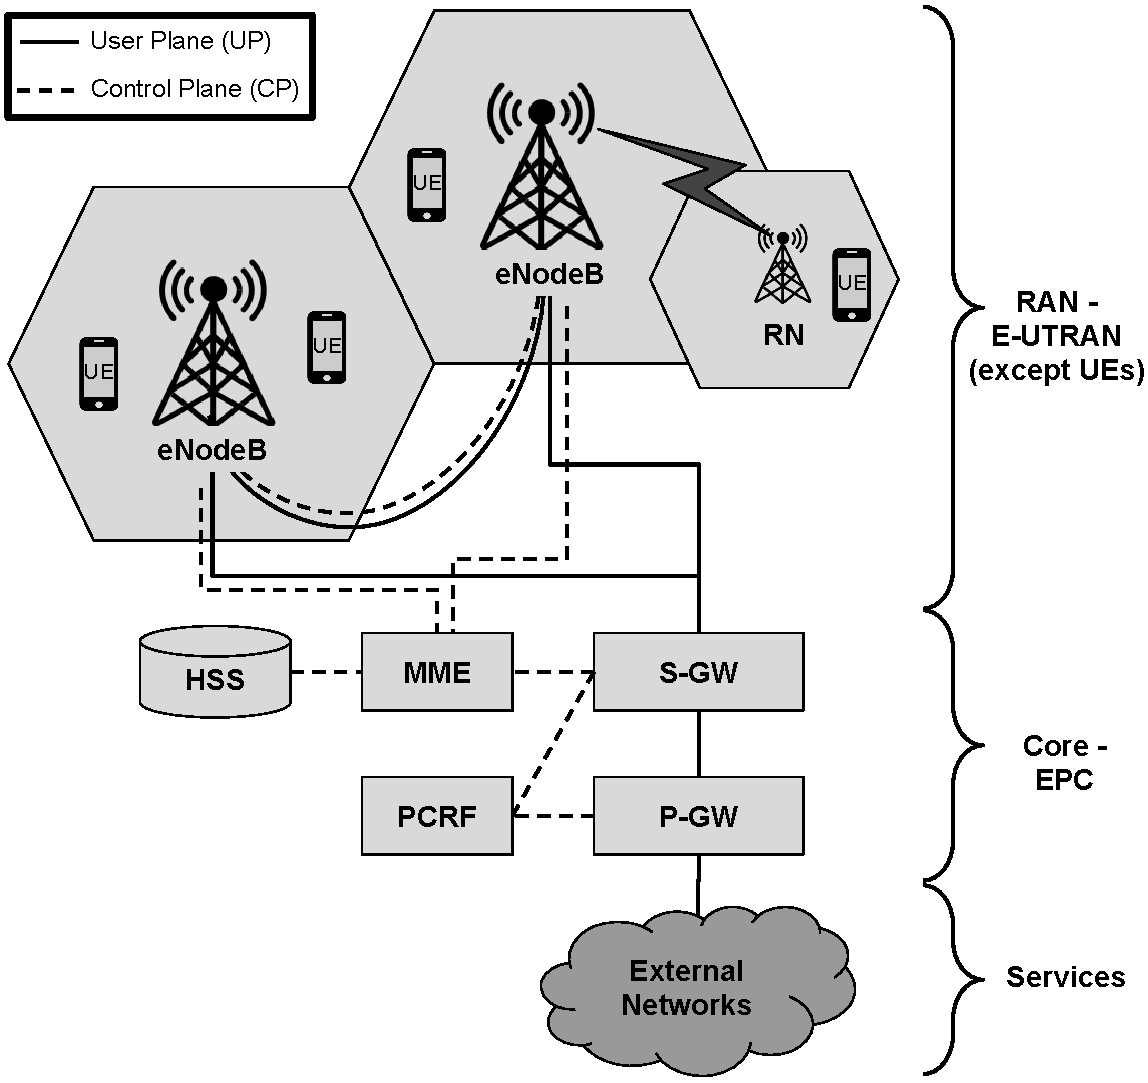
\includegraphics[width=0.5\textwidth]{figs/LTE-adv.pdf}
  \end{center}
\caption{System architecture of EPS with E-UTRAN only.}
\label{fig:lte-adv}
\end{figure}

A fundamental change in the architecture of the 4G core networks is the absence of circuit switching, \textit{i.e.}, the EPC does
not have direct connectivity to traditional circuit-switched networks, such as Integrated Services Digital Network (ISDN) or PSTN. As a consequence, voice communication is transported over IP or, more recently, over LTE until the core. The main components of the EPC are the following:

\begin{itemize}
\item Mobility Management Entity (MME) -- This is the main control element in the EPC and operates only in the Control Plane (CP). The MME is involved in authentication, security, mobility management (tracking, paging, handover), management of subscription profile, and service connectivity (bearer setup). Since the first UE register to the network, MME is involved in the authentication process that can be repeated later, including periodically. MME is also responsible for security measures such as ciphering, generation of integrity protection keys, and allocation of temporary identity to the UE. Moreover, to store and update UE-related data, mobility management involves the MME participating in the control signaling with eNodeBs and S-GWs, eventually, with other MMEs. During the time that the MME is serving a UE, it stores a temporary copy of the subscriber profile associated with UE. This profile contains the information that MME needs to adequately assist UE, for example, to set up the bearers to transport the services requested by UE.

\item Home Subscriber Server (HSS) -- This is the data repository for all permanent user data, such as a master copy of the subscriber profile and the permanent key used to calculate the authentication vectors. Some temporary data may be stored in HSS, such as the location of the user in the level of the visited network (\textit{i.e.}, when UE changes of MME) and identities of those P-GWs in use if the support for mobility between non-3GPP access networks is active.

\item Policy and Charging Rules Function (PCRF) -- This network element is responsible for Policy and Charging Control (PCC). Basically, PCRF makes decisions on how to handle the services in terms of QoS and provides the necessary information to the P-GW and, if applicable, also to the S-GW, so that appropriate bearers and policing can be set up.

\item Packet Data Network (PDN) Gateway (P-GW) -- This is the interconnection point between EPC and external networks (\textit{e.g.}, the Internet). P-GW performs traffic shaping and filtering functions according to policies defined for each UE and service. P-GW also collects and reports the related charging information and, typically, allocates the IP address to UEs.

\item Serving Gateway (S-GW) -- This is the interconnection point between RAN and EPC. The main functions of S-GW are User Plane (UP) tunnel management and switching. S-GW is minimally involved in control functions, being responsible for its resources that are allocated based on requests from MME, P-GW, or PCRF.
\end{itemize}